


\chapter{Numerical Results}
  \label{ch_results}

\todo{An overarching motivation for the present work is that FLRs exhibit significant behavioral changes as a result of their azimuthal modenumbers, but that prior models have been unable to provide a good picture. }

% -----------------------------------------------------------------------------
% -----------------------------------------------------------------------------
% -----------------------------------------------------------------------------
\section{Modenumber and Compression}
  \label{sec_compression}

It's well known that the poloidal FLR mode is compressional at low modenumber, but guided at high modenumber. However, the relationship is not well quantified. Theoretical work has historically been concerned with the limits $\azm \rightarrow 0$ and $\azm \rightarrow \infty$\cite{cummings_1969,radoski_1974}, and only a handful of satellite observations have explicitly considered an event's azimuthal modenumber\cite{dai_2013,motoba_2015,takahashi_2013}. Using results from Tuna, the present section examines the strength of the poloidal wave's compressional component at an ensemble of finite modenumbers. 

\cref{fig_snapshot_smallm,fig_snapshot_bigm} show magnetic field snapshots taken from a pair of runs. The first uses a small azimuthal modenumber, and the second uses a large one. The runs are otherwise identical: both simulations use the quiet dayside ionospheric profile, and both are driven at \SI{22}{\mHz}. 

\begin{figure}[!htb]
    \centering
    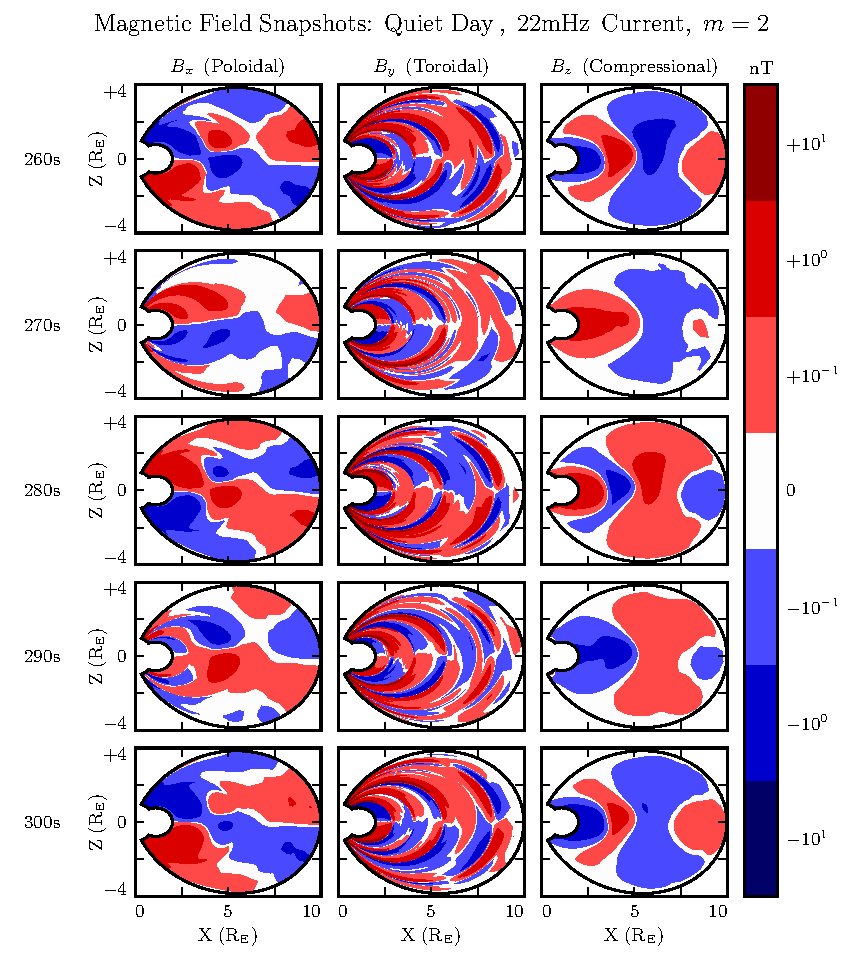
\includegraphics[width=\textwidth]{figures/snapshot_smallm.pdf}
    \caption[Magnetic Field Snapshots from a Small-\azm Run]{
      Each row in the above figure is a snapshot in time. The three columns show the simulated poloidal, toroidal, and compressional magnetic field. Due to the run's low azimuthal modenumber, the poloidal mode has a significant compressional component. This is visible both in the fact that $B_z$ is comparable in size to $B_x$, and in that structure in $B_x$ is only vaguely guided by the geometry of the magnetic field. Toroidal waves, in contrast, are sharply guided. 
    }
    \label{fig_snapshot_smallm}
\end{figure}

\begin{figure}[!htb]
    \centering
    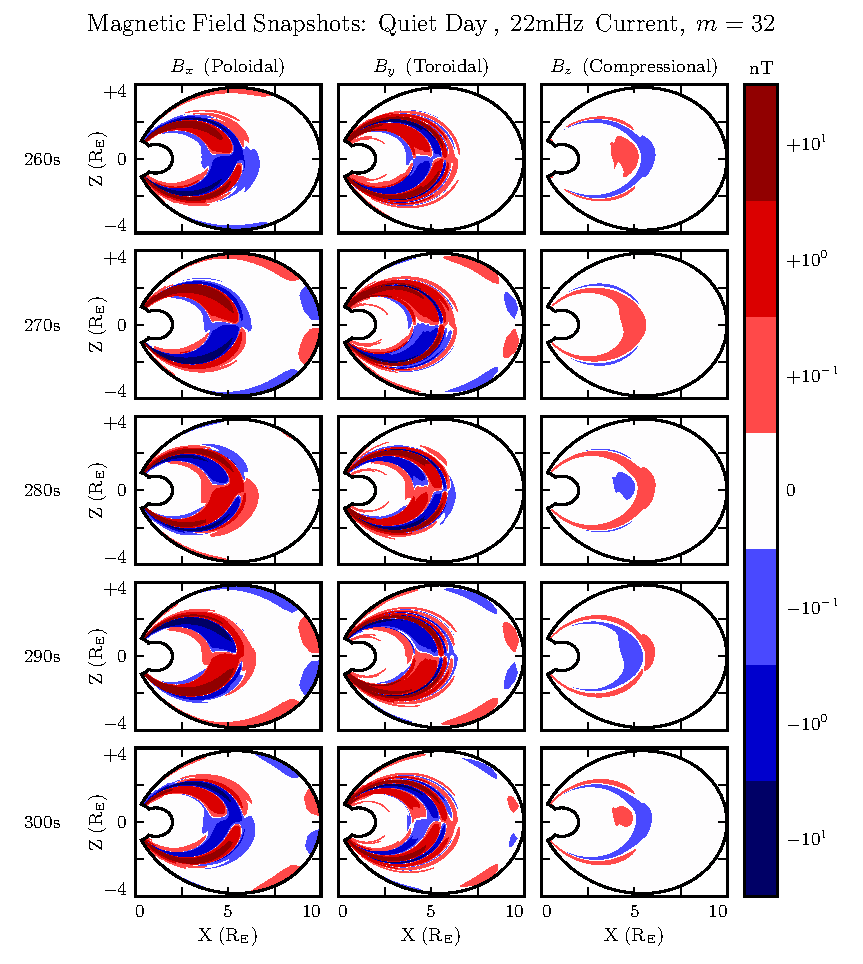
\includegraphics[width=\textwidth]{figures/snapshot_bigm.pdf}
    \caption[Magnetic Field Snapshots from a Large-\azm Run]{
      The above figure is analogous to \cref{fig_snapshot_smallm}, but the runs use a larger azimuthal modenumber. The change has a dramatic effect. The poloidal wave is concentrated much more sharply in $L$, and its compressional component is weakener by an order of magnitude. Regardless of modenumber, toroidal waves exist at a range of $L$ shells similar to poloidal waves, and show sharp definition across $L$-shells. 
    }
    \label{fig_snapshot_bigm}
\end{figure}

The differences between the two runs are striking. At low modenumber, wave activity is visible throughout the simulation domain. Structure in the poloidal magnetic field is only vaguely governed by the dipole geometry, and the compressional magnetic field is comparably strong to the two perpendicular components. 

In contrast, at high modenumber, the poloidal magnetic field is localized to the $L$-shells where the driving is delivered: $4 \lesssim L \lesssim 6$. The compressional field is weaker than the poloidal field by at least an order of magnitude. A third-harmonic poloidal mode is visible at the outer boundary --- its magnitude is just barely large enough to be visible on the logarithmic scale. The gap between $L\sim5$ (where \SI{22}{\mHz} matches a first-harmonic FLR) and $L\sim10$ (where \SI{22}{\mHz} matches a third-harmonic FLR) speaks to the evanescence of non-guided waves above the compressional \Alfven cutoff frequency\footnote{See \cref{sec_implications}. }. 

In both the low-\azm and high-\azm runs, toroidal activity is more or less coincident with poloidal activity --- as is to be expected, since the driving is purely poloidal, and the poloidal mode rotates to the toroidal mode over time. It is further notable that the toroidal mode is sharply guided. Particularly in \cref{fig_snapshot_bigm}, strong, narrow, toroidal FLRs of opposite phase can be seen oscillating very close to one another. Strong poloidal waves, in contrast, are smeared in $L$. 

Snapshots are not shown for runs carried out using the other ionospheric profiles (active day, quiet night, and active night). The morphology of their waves is qualitatively similar. The differences between the profiles is considered in \cref{sec_day,sec_night,sec_ground}. 

\begin{figure}[!htb]
    \centering
    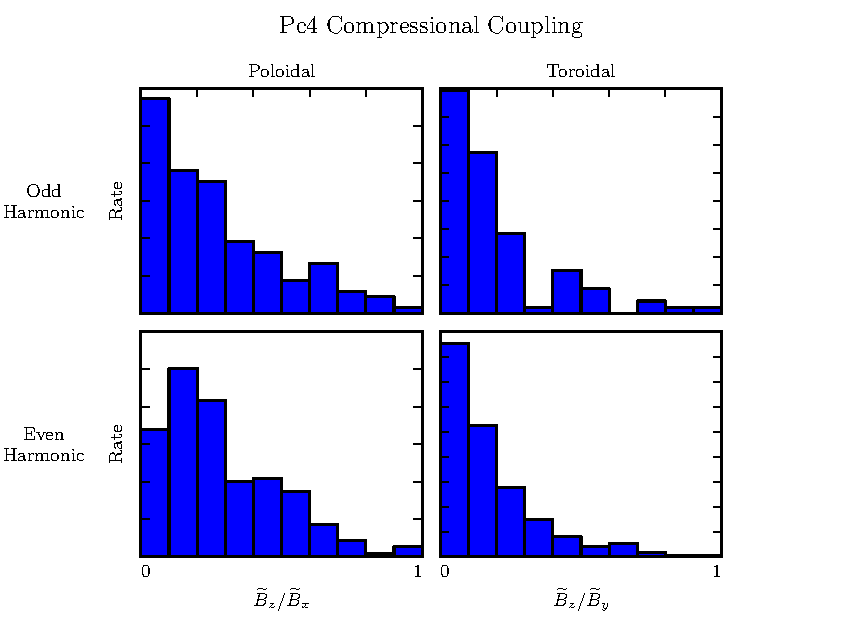
\includegraphics[width=\textwidth]{figures/comp.pdf}
    \caption[Compressional Coupling to the Poloidal Mode]{
      Each subplot above corresponds to a different run; the runs shown in \cref{fig_snapshot_smallm,fig_snapshot_bigm} are in the rightmost column, second from the top and second from the bottom respectively. Red lines indicate the ratio between the RMS compressional and poloidal magnetic fields. Mean values are shown in black. The compressional field is comparable to the poloidal field at $\azm = 1$, but falls quickly. 
    }
    \label{fig_comp}
\end{figure}

\cref{fig_comp} quantifies the compressional component of the poloidal mode as a function of modenumber. Each subplot corresponds to a different run of Tuna --- the runs shown in \cref{fig_snapshot_smallm,fig_snapshot_bigm} are in the rightmost column, second from the top and second from the bottom respectively. The red line indicates the ratio between the RMS compressional magnetic fieldand the RMS poloidal magnetic field; both averages are taken over the entire simulation ``volume'' each time step. Mean values are shown in black. 

At $\azm = 1$, the compressional and poloidal magnetic fields are comparable in magnitude. As \azm increases, however, the compressional component quickly falls off. The compressional component is half the strength of the poloidal component at $\azm \sim 5$, and a quarter by $\azm \sim 10$. 

A slight frequency dependence is apparent across each row in \cref{fig_comp}. Compressional coupling falls off slower for waves at higher frequency. This is because higher-frequency waves are that much closer to the cutoff frequency (described in \cref{sec_implications}), and so their propagation across $L$-shells is that much less evanescent. 

Similarly, poloidal waves are more prone to compression on the nightside. Due to the higher \Alfven speed on the nightside, driving is delivered at $L \sim 6$ instead of $L \sim 5$. The cutoff frequency depends inversely on radial distance. For nightside runs (not shown), $\left| \frac{B_z}{B_x} \right|$ falls to \SI{50}{\percent} at $\azm \sim 8$ and to \SI{25}{\percent} at $\azm \sim 16$. 

Notably, the waves considered in the present work are fundamental harmonics. The compressional behavior of the poloidal mode may vary for the (more-common) second harmonic: Radoski suggests that the asymptotic value of $\left| \frac{B_z}{B_x} \right|$ is inversely proportional to the harmonic number\cite{radoski_1974}. 

%\todo{Results might vary significantly for even modes. Radoski's 1974 paper suggests that $\left|\frac{B_z}{B_x}\right|\sim\frac{1}{n}$ (where $n$ is the harmonic number). }

%\todo{The nature of the relationship between \azm and the compressional coupling is not obvious. It's not linear, logarithmic, or a power law. }

%\todo{These results line up nicely with Dai's 2015 survey of poloidal Pc4 events\cite{dai_2015}. Events are characterized as compressional or non-compressional based on the ratio $\left|\frac{B_z}{B_x}\right|$. The threshold is arbitrarily set to \num{0.2} --- with no suggestion of a corresponding value of \azm. The results in \cref{fig_comp_2} suggest that Dai's threshold (conveniently!) aligns closely with the paper's definition of ``small \azm'' to mean $\azm < 10$. }

%\todo{Check if a relationship is given in Hughes\cite{hughes_1994}. That's what Lei cites for ``low-\azm waves are compressional.'' Other papers give no indication that this has been looked at before\cite{cummings_1969,radoski_1974}. }

% -----------------------------------------------------------------------------
% -----------------------------------------------------------------------------
% -----------------------------------------------------------------------------
\section{Resonance and Rotation on the Dayside}
  \label{sec_day}

In his 1974 paper, Radoski argues that a poloidally-polarized wave should asymptotically rotate to the toroidal polarization\cite{radoski_1974} as a result of the curved derivative in the meridional plane. The question of finite poloidal lifetimes is considered further in a 1995 paper by Mann and Wright\cite{mann_1995}. Their numerical work used a straightened field line, with an \Alfven speed gradient in the ``radial'' direction. They also found a rotation over time from poloidal to toroidal polarization, with the characteristic time proportional to the azimuthal modenumber. 

The present section builds on the aforementioned results by relaxing several of their nonphysical assumptions. Tuna's geometry is more realistic than Radoski's half-cylinder or the box model usede by Mann and Wright. Previous work has considered the evolution of an initial condition, while the simulations shown below include driving delivered over time. In addition, Tuna features a finite, height-resolved ionospheric conductivity profile, rather than the perfectly-reflecting boundaries used in the past. 

Each subplot in \cref{fig_U_day} is analogous to Figure 3 in Mann and Wright's paper\cite{mann_1995}. Blue lines show the total energy in the poloidal mode as a function of time. Red lines show toroidal energy. Runs are organized analogous to those in \cref{fig_comp}: drive frequency is constant down each column, and azimuthal modenumer is constant across each row. Axis bounds are held constant across all subplots. The poloidal and toroidal energy are computed by integrating over the electromagnetic energy density, per Poynting's theorem:
\begin{align}
  \label{def_energy}
  U_P &= \displaystyle\int \frac{dV}{2 \mz} \lr{ B_x^2 + \frac{1}{\va^2} E_y^2} &
  U_T &= \displaystyle\int \frac{dV}{2 \mz} \lr{ B_y^2 + \frac{1}{\va^2} E_x^2} 
\end{align}

Where the differential volume $dV$ is computed using the Jacobian\footnote{See \cref{sec_coords}. } to account for Tuna's unusual geometry. The integral is evaluated in \lysakx and \lysakz but not \lysaky (Tuna's missing half-dimension), which gives energy in units of gigajoule per radian. More than anything else, this serves as a reminder that Pc4 pulsations are localized in MLT. 

\begin{figure}[!htb]
    \centering
    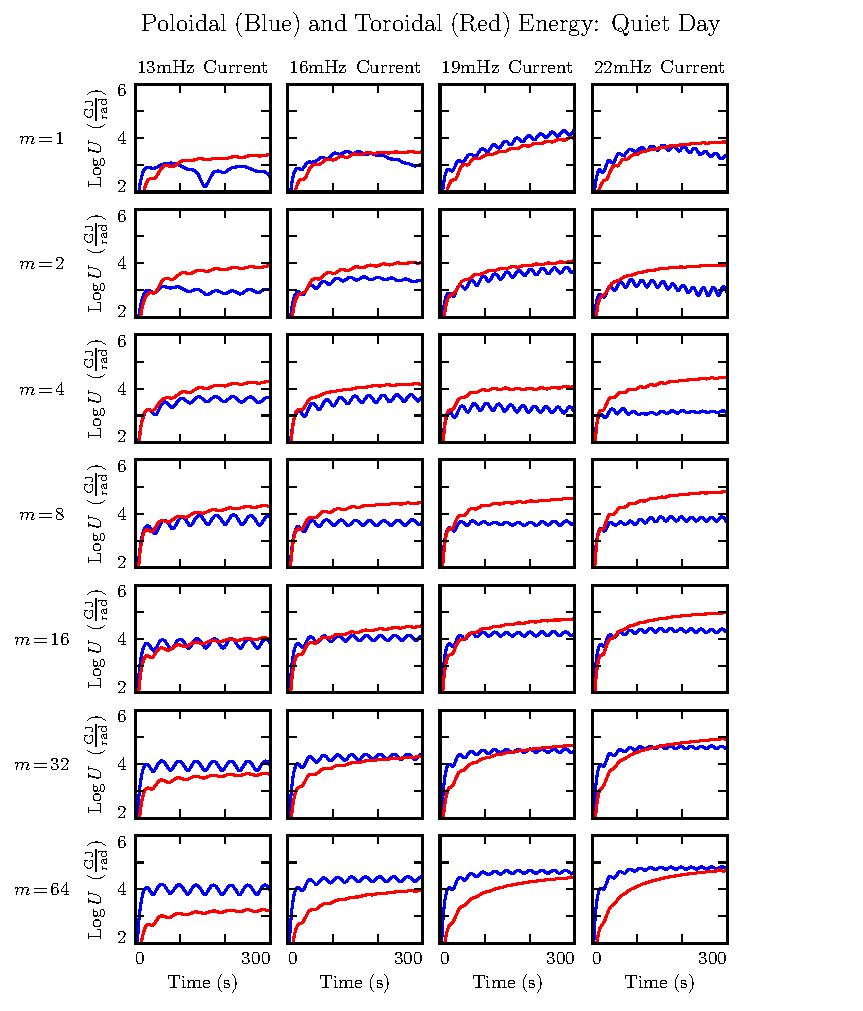
\includegraphics[width=\textwidth]{figures/U_day.pdf}
    \caption[Dayside Poloidal and Toroidal Energy]{
      \todo{Lorem ipsum dolor sit amet, consectetur adipiscing elit, sed do eiusmod tempor incididunt ut labore et dolore magna aliqua. Ut enim ad minim veniam, quis nostrud exercitation ullamco laboris nisi ut aliquip ex ea commodo consequat. Duis aute irure dolor in reprehenderit in voluptate velit esse cillum dolore eu fugiat nulla pariatur. }
    }
    \label{fig_U_day}
\end{figure}

The 28 runs shown in \cref{fig_U_day} use an ionospheric profile corresponding to the dayside during times of low solar activity, where the conductivity is relatively high. The active and quiet dayside profiles are briefly contrasted in \cref{sec_ground}; for the most part, the focus of the present work is on the difference between the dayside and the nightside (\cref{sec_night}). Differences between the two dayside profiles are small in comparison. 

The fact that red (toroidal) lines appear at all in \cref{fig_U_day} speaks to a net rotation of energy from the poloidal mode to the toroidal. As discussed in \cref{sec_driving}, Tuna's driving is delivered purely into the poloidal electric field (reflecting a perturbation in the magnitude of the ring current). 

As expected, the rotation from poloidal to toroidal is slowest at large azimuthal modenumbers. The toroidal energy overtakes the poloidal energy within a single drive period at $\azm=4$; at $\azm=64$, the most of the energy is in the poloidal mode for \about10 periods. However, the relationship between azimuthal modenumber and rotation timescale is not linear, as was suggested by Mann and Wright. Instead, in a practical setting, the rotation is fastest at $\azm \sim 4$. 

This is explained by the compressional character of the poloidal mode. At very low modenumber, energy in the poloidal mode moves readily across $L$-shells. A significant fraction of that energy is lost to the outer boundary before rotating to the toroidal mode. At high modenumber --- as discussed in \cref{sec_compression} --- compressional propagation is evanescent, so all energy in the poloidal mode must ultimately rotate to the toroidal mode or be lost to Joule dissipation. 

Joule dissipation is a major player in the system's energy economy. However, due to the highly conductive dayside ionosphere, dissipation timescales are in the tens of Pc4 wave periods. Energy loss through Joule dissipation asymptotically balances energy input from driving, but most of that energy is not lost until after it has rotated from the poloidal mode to the toroidal. As such, in most runs shown in \cref{fig_U_day}, the energy content of the toroidal mode asymptotically exceeds that of the poloidal mode. 

The asymptotic energy content of the system also depends on how well the drive frequency matches the local eigenfrequency. If the two do not match, energy is lost to destructive interference between the standing wave and the driving. 

In principle, energy moves between the poloidal and toroidal modes due to their direct coupling through the ionospheric Hall conductivity. In practice, this effect is small. When the runs shown in \cref{fig_U_day} are repeated with the Hall conductivity set to zero, the resulting energy curves are not visibly different. 

The low-\azm runs at \SI{19}{\mHz} merit additional discussion. These runs accumulate energy over a large number of wave periods, while the low-\azm waves at \SI{13}{\mHz}, \SI{16}{\mHz}, and \SI{22}{\mHz} do not. This effect is likely nonphysical. At \SI{19}{\mHz}, a third-harmonic resonance forms very close to the outer boundary. The resonance is likely enhanced by nonphysical reflections against the simulation's boundary conditions. 

The presence of individual harmonics can be seen in the contours shown in \cref{fig_layers_day_p,fig_layers_day_t}. These figures show the same runs as \cref{fig_U_day}, arranged in the same way on the page. However, instead of showing the total energy integrated over the simulation domain, the energy densities are averaged over the volume of each flux tube individually. \cref{fig_layers_day_p} shows contours of poloidal energy density and \cref{fig_layers_day_t} shows toroidal energy density. 

\begin{figure}[!htb]
    \centering
    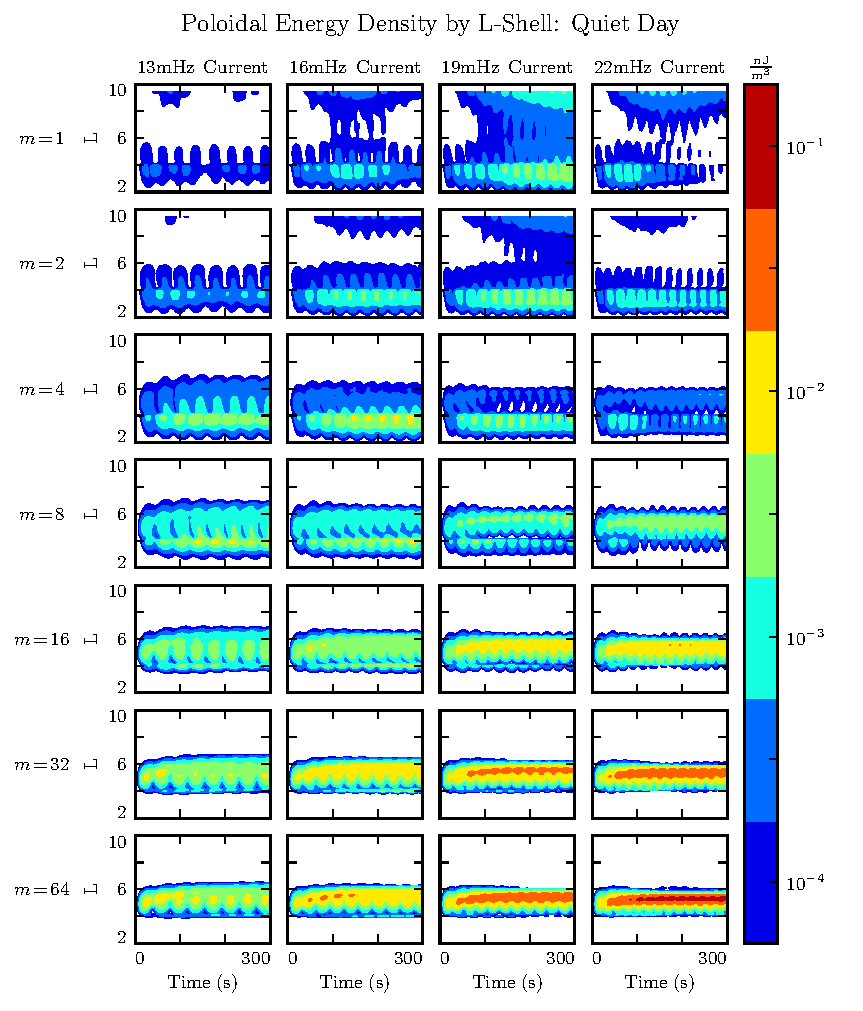
\includegraphics[width=\textwidth]{figures/layers_day_p.pdf}
    \caption[Dayside Poloidal Energy Distribution]{
      \todo{Lorem ipsum dolor sit amet, consectetur adipiscing elit, sed do eiusmod tempor incididunt ut labore et dolore magna aliqua. Ut enim ad minim veniam, quis nostrud exercitation ullamco laboris nisi ut aliquip ex ea commodo consequat. Duis aute irure dolor in reprehenderit in voluptate velit esse cillum dolore eu fugiat nulla pariatur. }
    }
    \label{fig_layers_day_p}
\end{figure}

\begin{figure}[!htb]
    \centering
    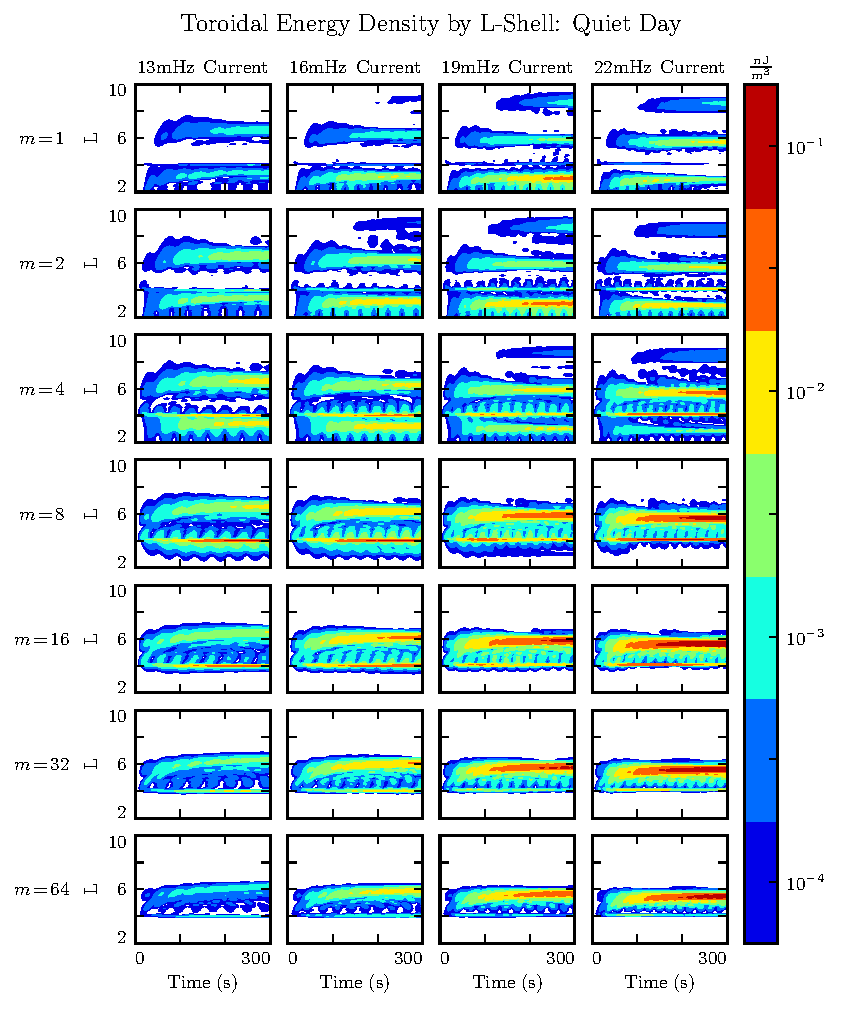
\includegraphics[width=\textwidth]{figures/layers_day_t.pdf}
    \caption[Dayside Toroidal Energy Distribution]{
      \todo{Lorem ipsum dolor sit amet, consectetur adipiscing elit, sed do eiusmod tempor incididunt ut labore et dolore magna aliqua. Ut enim ad minim veniam, quis nostrud exercitation ullamco laboris nisi ut aliquip ex ea commodo consequat. Duis aute irure dolor in reprehenderit in voluptate velit esse cillum dolore eu fugiat nulla pariatur. }
    }
    \label{fig_layers_day_t}
\end{figure}

The top few rows of \cref{fig_layers_day_p} confirm that the poloidal mode's compressional nature is to blame for its failure to accumulate energy at low modenumber. Waves move so readily across field lines that no visible amount of energy builds up at $L \sim 5$, the location of the driving. Some energy moves inward, and is trapped by the peak in \Alfven speed just inside the plasmapause, while the rest moves to the outer boundary. The time spent moving across field lines counts against the poloidal mode's finite lifetime, inhibiting the buildup of poloidal energy density even at $L$-shells where the wave matches the local eigenfrequency. 

As \azm increases, the energy distribution becomes more concentrated in $L$, though individual features remain fairly broad. At $\azm = 8$, runs at \SI{13}{\mHz} and \SI{16}{\mHz} are inclined to build up energy just inside the plasmapause, while those at \SI{19}{\mHz} and \SI{22}{\mHz} resonate just outside the plasmapause; in all four cases, the energy is spread over a range of at least 1 in $L$. 

The peak energy density in the bottom-right run (\SI{22}{\mHz} driving, $\azm = 64$) is by far the largest of any run in \cref{fig_layers_day_p}. The azimuthal modenumber is large, so the poloidal mode is purely guided; energy is not smeared across multiple $L$-shells. And, crucially, the frequency of the driving  matches closely with the \Alfven frequency at $L \sim 5$. Other runs on the bottom row are also guided, but they reach lower asymptotic energy densities because of a mismatch between the drive frequency and the local eigenfrequency --- resulting in destructive interference between the standing wave and its driver. 

The eigenfrequencies in the magnetosphere are significantly affected by the location of the plasmapause. When the runs in \cref{fig_layers_day_p} are repeated with the plasmapause at $L = 5$ instead of $L = 4$, the strongest resonance at $L \sim 5$ drops from \SI{22}{\mHz} to \SI{16}{\mHz} (not shown). 

Whereas the poloidal contours are smeared over a swath of $L$-shells (though the high-\azm runs less so), the toroidal contours in \cref{fig_layers_day_t} appear only where the wave frequency matches the local eigenfrequency. A horizontal line drawn through the \Alfven speed frequency profiles (recall \cref{fig_fa}) intersects the profile up to three times: once as the \Alfven frequency drops through the Pc4 range from its low-latitude peak, again as the \Alfven frequency rises sharply at the plasmapause, and a third time as the \Alfven frequency drops asymptotically. Toroidal waves can be seen resonating at all three of these locations in the $\azm = 4$, \SI{22}{\mHz} run in \cref{fig_layers_day_t}, along with a third harmonic at large $L$. This is consistent with observations: toroidal resonances are noted for having frequencies which depend strongly on $L$, in contrast to the poloidal mode's less-strict relationship between frequency and location. 

In only one of the runs shown in \cref{fig_layers_day_p} does the poloidal mode attain an energy density on the order of \SI{e-1}{\nJ/\meter\cubed}. On the other hand, the toroidal mode reaches \about\SI{e-1}{\nJ/\meter\cubed} in six of the runs in \cref{fig_layers_day_t}. That is, the poloidal mode only exhibits a high energy density on the dayside only when conditions are ideal; the toroidal mode isn't nearly so particular. 

% -----------------------------------------------------------------------------
% -----------------------------------------------------------------------------
% -----------------------------------------------------------------------------
\section{Resonance and Rotation on the Nightside}
  \label{sec_night}

\todo{ACTUALLY we should show the runs driven at $L\sim5$ across the board. Dayside and nightside. That way we can make a fair comparison. }




Compared to the dayside ionosphere employed in \cref{sec_day}, the nightside exhibits two major differences. The ionospheric conductivity is lower, and the \Alfven speed is higher. As a result of the higher \Alfven speed, driving on the nightside is delivered at $L \sim 6$ instead of $L \sim 5$. Runs in the present section specifically use Tuna's ionospheric profile corresponding to the nightside during quiet solar conditions; the active nightside is discussed briefly in \cref{sec_ground}, but for the most part the present work is concerned with the behavior of the nightside compared to that on the dayside. 

Other than the change in ionospheric profile, \cref{fig_U_night,fig_layers_night_p,fig_layers_night_t} are analogous to \cref{fig_U_day,fig_layers_day_p,fig_layers_day_t}. Each subplot corresponds to a different \SI{300}{\s} run of Tuna. Drive frequency is constant down each column, and azimuthal modenumber is constant across each row. 

The low conductivity on the nightside gives rise to strong Joule dissipation. Waves are damped out in just a few bounces, so asymptotic energy values are reached quickly. No combination of frequency and modenumber gives rise to the accumulation of energy over multiple drive periods. 

As on the dayside, rotation of energy from the poloidal to toroidal mode is fastest at $\azm \sim 4$. Unlike the dayside, however, dissipation on the nightside is fast compared to the rotation of energy to the toroidal mode. Toroidal energy does not asymptotically exceed the poloidal energy by a significant margin in any run. At $\azm = 64$, where the rotation timescale is slowest, no more than \todo{$\cdots$} of the energy in the poloidal mode rotates to the toroidal mode before being lost. 

\todo{The damping on the quiet nightside is so severe that basically nothing resonates anywhere. Should we show the active nightside instead? }


%There is surprisingly little difference between \todo{$\cdots$} (the subplots of which are arranged analogously). Asymptotic energy levels vary --- in the case of high \azm and low frequency, runs in \todo{$\cdots$} are more energetic by an order of magnitude or more --- but the qualitative behavior is the same. Driving is balanced by dissipation over the course of just a few drive periods. Dissipation outstrips poloidal-to-toroidal rotation in the case of large azimuthal modenumber. And, unlike on the dayside, the toroidal mode typically does not match the asymptotic energy level seen in the poloidal mode. 

%\todo{$\cdots$} shows the radial distribution of poloidal energy on the nightside --- a slice of each run shown in \todo{$\cdots$}. Broadly speaking, the behavior is consistent with that seen in \todo{$\cdots$}: energy is smeared across $L$-shells at small \azm and guided at high \azm, with particularly strong energy buildup when the drive frequency matches the local \Alfven frequency. 

%As discussed in \todo{$\cdots$}, the nightside's relatively low ionospheric conductivity increases the rate of dissipation. Asymptotic energy content is reached quickly, and is small compared to that seen in analogous dayside runs. 

%The effect is particularly pronounced at large modenumber, where the poloidal-to-toroidal rotation timescale is slower than the nightside dissipation timescale. In most of the dayside runs shown in \todo{$\cdots$}, the toroidal mode asymptotically exceeds the poloidal mode both in terms of total energy content and in terms of peak energy density. On the nightside, the opposite is true. At high modenumber, the asymptotic rotation from the poloidal mode to the toroidal mode doesn't occur until most of the energy has been lost to Joule dissipation. Peak poloidal energy densities at $\azm = 64$ exceed their toroidal counterparts --- shown in \todo{$\cdots$} --- by an order of magnitude. 

%\todo{On the nightside, unlike the dayside, toroidal contours are messy. Why? }

%The behavior of the poloidal mode on the nightside matches qualitatively with the behavior on the dayside. At low \azm, energy is lost to the outer boundary. At high \azm, resonance occurs, but only if the drive frequency is close to the local eigenfrequency. The big difference is that, due to the increased dissipation in the ionopshere, asymptotic energy densities are relatively low, and reached relatively quickly. 

%In low-\azm runs, the poloidal mode loses energy to the outer boundary, which impairs the growth of the toroidal mode. At high \azm, poloidal-to-toroidal rotation is slow compared to dissipative timescales on the nightside. The strongest toroidal waves --- which are still weak compared to those on the dayside --- thus appear at moderate \azm. 

%\todo{$\cdots$} is arranged analogously to the figures in \cref{sec_day}: each subplot is an independent run, drive frequency is constant down each column, and azimuthal modenumber is constant across each row. Poloidal energy is blue; toroidal energy is red. 

%The lower energies in \todo{$\cdots$} (compared to \todo{$\cdots$}, the analogous dayside runs) are not entirely due to increased Joule dissipation. Due to the difference in electric constant between the dayside and nightside magnetospheres\footnote{See \cref{fig_fa}. }, resonant frequencies just outside the typical ($L_{PP} = 4$) plasmapause fall well outside the Pc4 range. None of the frequencies shown in \todo{$\cdots$}, when delivered at $L_{drive} = 5$, align with the local eigenfrequency. 

%As in \todo{$\cdots$}, the \SI{19}{\mHz} run with $\azm = 1$ is an apparent exception. A large amount of energy builds up in a third harmonic very close to the outer boundary. The interaction is likely nonphysical. 

%\todo{It may be significant that $\int \sigma dz$ is constant across all $L$-shells, but $\int \frac{\sigma}{\va^2} dz$ is not. }

%Behavior closer to resonance is shown in \todo{$\cdots$}. The plasmapause remains at $L_{PP} = 4$, but the driving is moved out to $L_{drive} = 6$, at which point the local \Alfven frequency overlaps the Pc4 frequency band. 

%Each subplot in \cref{fig_U_night,fig_layers_night_p,fig_layers_night_t} corresponds to a run. 


\begin{figure}[!htb]
    \centering
    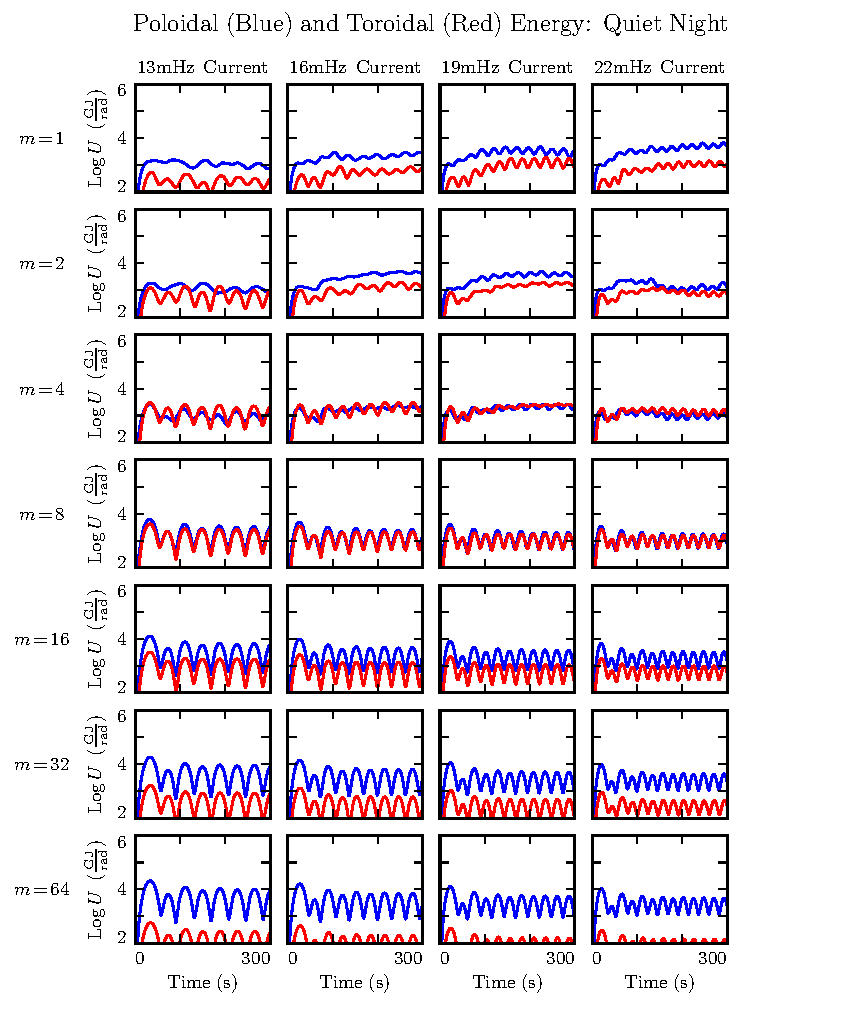
\includegraphics[width=\textwidth]{figures/U_night.pdf}
    \caption[Nightside Poloidal and Toroidal Energy]{
      \todo{Lorem ipsum dolor sit amet, consectetur adipiscing elit, sed do eiusmod tempor incididunt ut labore et dolore magna aliqua. Ut enim ad minim veniam, quis nostrud exercitation ullamco laboris nisi ut aliquip ex ea commodo consequat. Duis aute irure dolor in reprehenderit in voluptate velit esse cillum dolore eu fugiat nulla pariatur. }
    }
    \label{fig_U_night}
\end{figure}


\begin{figure}[!htb]
    \centering
    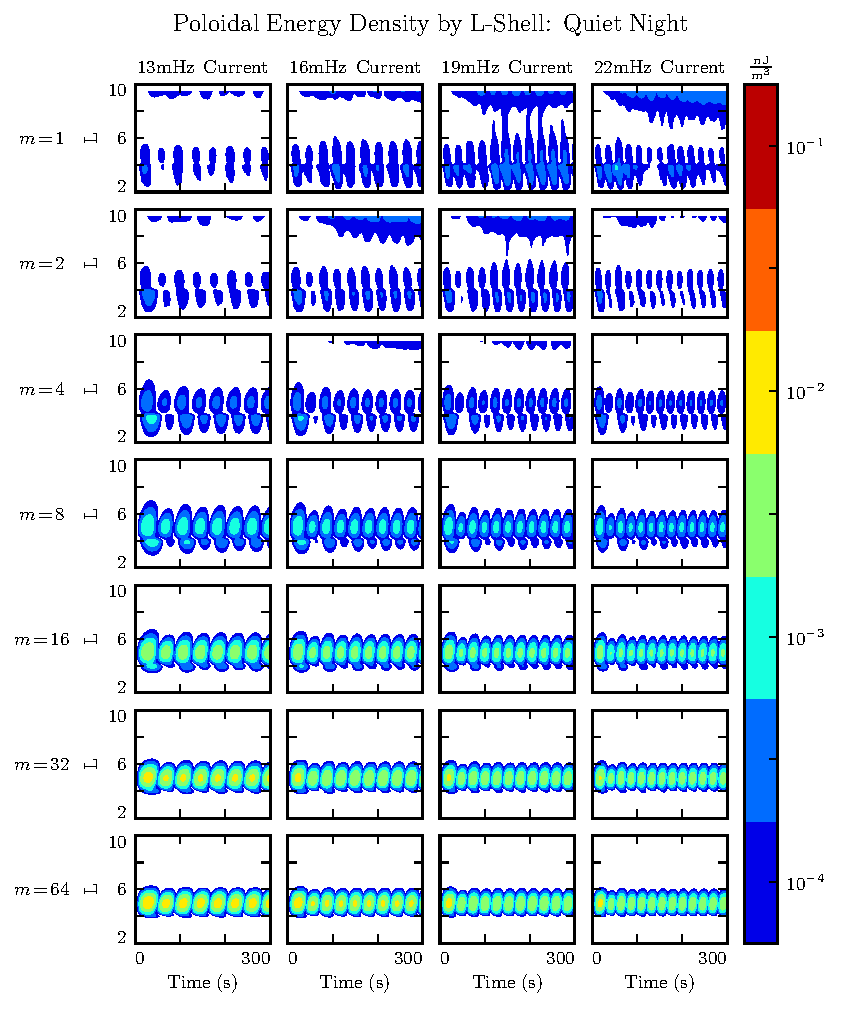
\includegraphics[width=\textwidth]{figures/layers_night_p.pdf}
    \caption[Nightside Poloidal Energy Distribution]{
      \todo{Lorem ipsum dolor sit amet, consectetur adipiscing elit, sed do eiusmod tempor incididunt ut labore et dolore magna aliqua. Ut enim ad minim veniam, quis nostrud exercitation ullamco laboris nisi ut aliquip ex ea commodo consequat. Duis aute irure dolor in reprehenderit in voluptate velit esse cillum dolore eu fugiat nulla pariatur. }
    }
    \label{fig_layers_night_p}
\end{figure}

\begin{figure}[!htb]
    \centering
    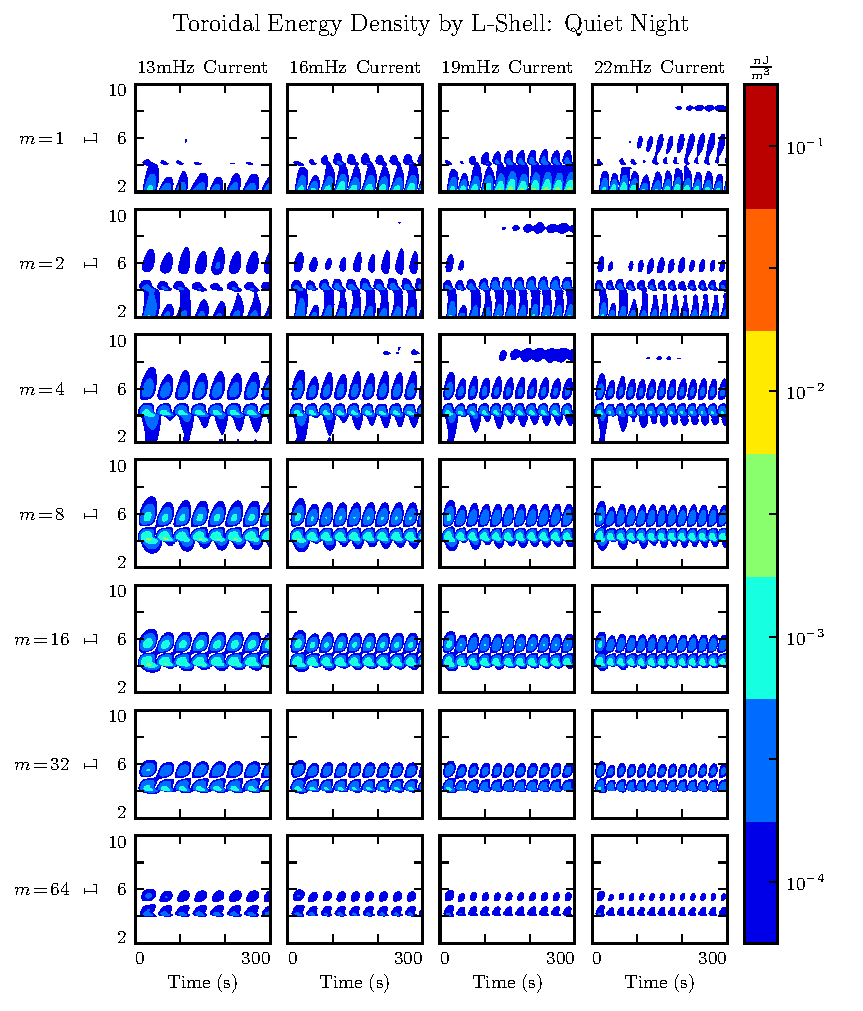
\includegraphics[width=\textwidth]{figures/layers_night_t.pdf}
    \caption[Nightside Toroidal Energy Distribution]{
      \todo{Lorem ipsum dolor sit amet, consectetur adipiscing elit, sed do eiusmod tempor incididunt ut labore et dolore magna aliqua. Ut enim ad minim veniam, quis nostrud exercitation ullamco laboris nisi ut aliquip ex ea commodo consequat. Duis aute irure dolor in reprehenderit in voluptate velit esse cillum dolore eu fugiat nulla pariatur. }
    }
    \label{fig_layers_night_t}
\end{figure}


% -----------------------------------------------------------------------------
% -----------------------------------------------------------------------------
% -----------------------------------------------------------------------------
\section{Ground Signatures and Giant Pulsations}
  \label{sec_ground}

While the majority of the action is in space, the majority of FLR observations have historically been ground-based. The present section explores the same simulations discussed in \cref{sec_day,sec_night}, but in terms of their ground signatures rather than their broad energy distributions. 

As in the figures shown in \cref{sec_day,sec_night}, each row in \cref{fig_ground_day,fig_ground_night} shows runs at a different modenumber. The columns are magnetic field contours; the vertical axis is latitude, and the horizontal axis is time. The four columns are components of the magnetic field signatures at the ground:  the north-south magnetic field (first and third columns) and the east-west magnetic field (second and fourth columns). The pair on the left show a simulation carried out using the active ionospheric profile, and the pair on the right show a simulation using the quiet profile. 

Notably, the magnetic polarization of a low frequency \Alfven wave is rotated by \about\SI{90}{\degree} as it passes through the ionosphere\cite{hughes_1974}. The east-west field on the ground ($B_\phi$) corresponds to the poloidal polarization in space, and the north-south field on the ground ($B_\theta$) corresponds to the toroidal mode. 

The most striking feature of \cref{fig_ground_day,fig_ground_night} is the modenumber dependence. As modenumber increases, the magnetic field signatures become sharply localized in latitude. At high \azm, ground signatures are concentrated between \SI{60}{\degree} and \SI{70}{\degree}, peaking near \SI{64}{\degree} on the dayside and \SI{66}{\degree} on the nightside. Appropriately enough, these latitudes lie at the $L\sim5$ and $L\sim6$ respectively. 

\todo{Is it weird that we see no ducting from the ionosphere? Does the ionosphere duct ULF waves in the $\theta$ direction, or just in $\phi$? }

At low modenumber, magnetic signatures are weak on the ground because the waves in space are also weak. At high modenumber, waves in space are strong, but so is the attenuation of magnetic signatures by the ionosphere\footnote{See \cref{attenuation}. }. The ``sweet spot'' at which magnetic ground signatures are maximized falls at $\azm = 16$ to $\azm = 32$. 

Tuna shows stronger ground signatures on the dayside than on the nightside, more or less in proportion with the difference in magnitude in space. Energy on the dayside (which depends on field magnitude squared) peaks an order of magnitude larger than that on the nightside. Peak ground signatures on the dayside are larger by a factor of five: \SI{45}{\nT} compared to \SI{10}{\nT}. On both the dayside and the nightside, peak ground signatures are in $B_\phi$, the east-west magnetic field component; both are also at $\azm = 16$, and both are seen in runs using the ionospheric profile for quiet solar activity. 

\todo{Check the other frequencies to make sure these are the real maxima. Probably also should print the maximum magnitude at the bottom of the subplot. }

These results match well with observations of giant pulsations, which tend to be east-west polarized, and are most often observed near \SI{66}{\degree}, with azimuthal modenumbers of 16 to 35, at the bottom of the solar cycle\cite{takahashi_1992}. Pgs are most commonly observed pre-dawn, but dawn and dusk ionospheric profiles are not implemented for Tuna at present. 

\begin{figure}[!htb]
    \centering
    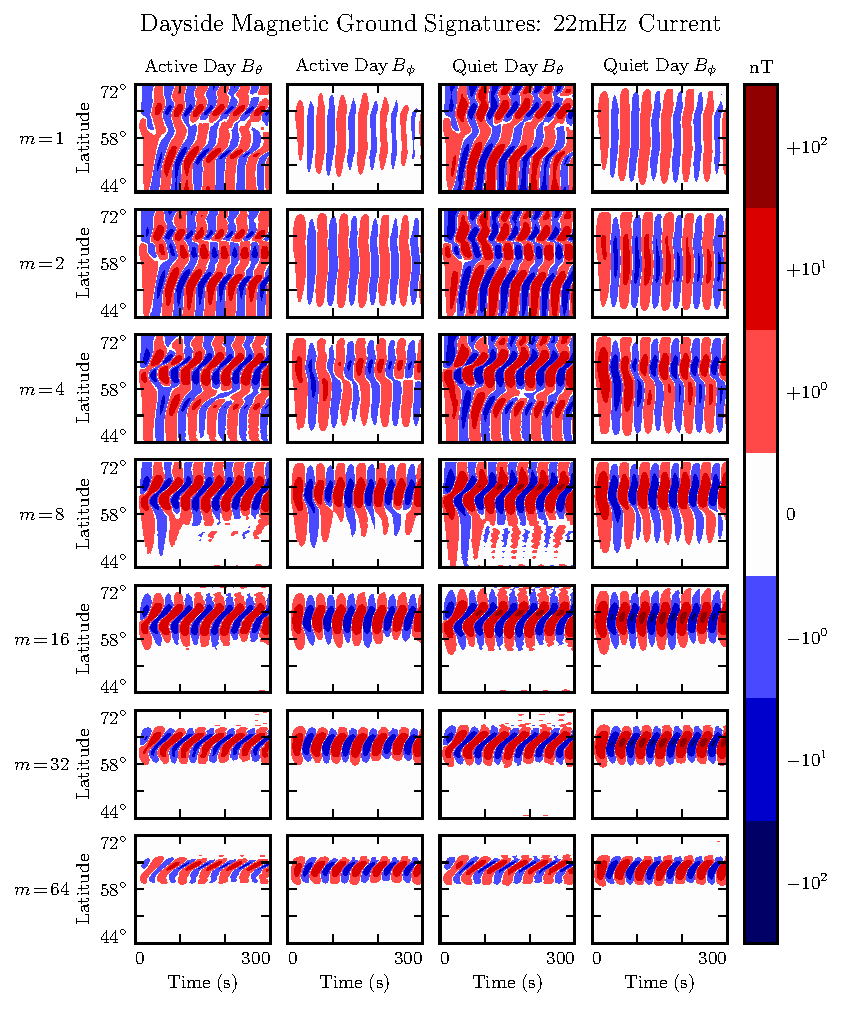
\includegraphics[width=\textwidth]{figures/ground_day.pdf}
    \caption[Dayside Ground Magnetic Fields]{
      \todo{Lorem ipsum dolor sit amet, consectetur adipiscing elit, sed do eiusmod tempor incididunt ut labore et dolore magna aliqua. Ut enim ad minim veniam, quis nostrud exercitation ullamco laboris nisi ut aliquip ex ea commodo consequat. Duis aute irure dolor in reprehenderit in voluptate velit esse cillum dolore eu fugiat nulla pariatur. }
    }
    \label{fig_ground_day}
\end{figure}

\begin{figure}[!htb]
    \centering
    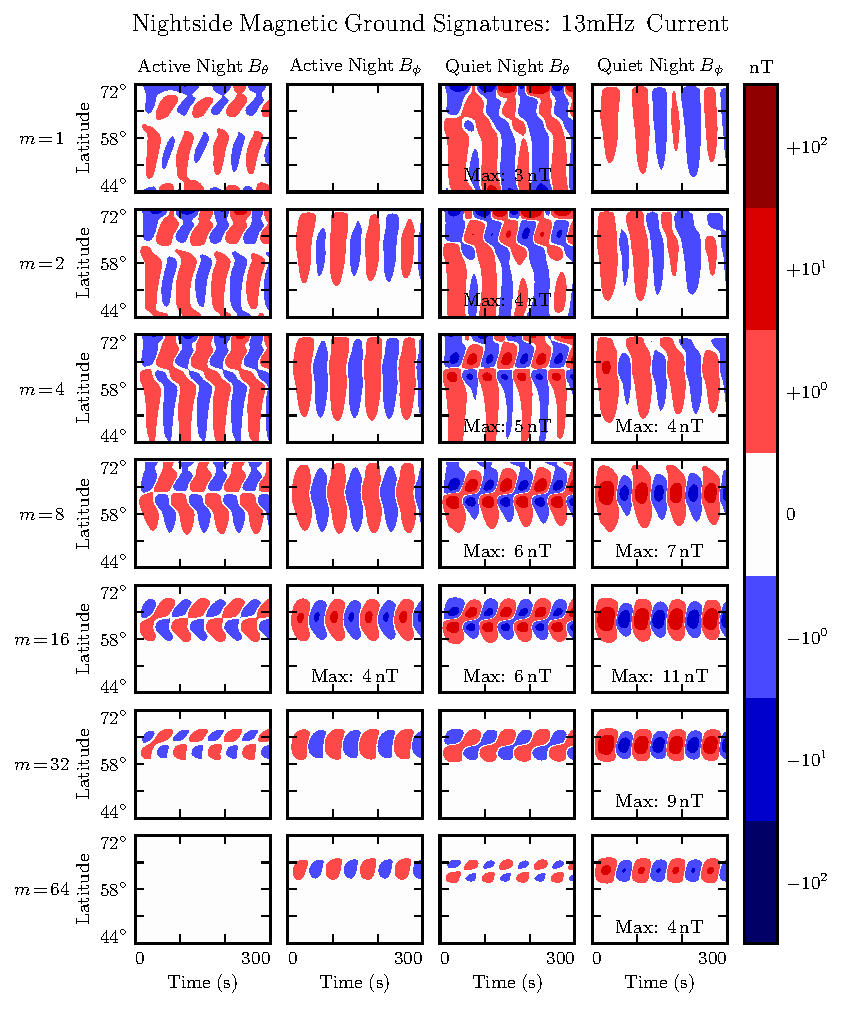
\includegraphics[width=\textwidth]{figures/ground_night.pdf}
    \caption[Nightside Ground Magnetic Fields]{
      Nightside ground signatures are less strongly peaked than those on the dayside, but qualitative features are the same: the strongest signals are in $B_\phi$, peaked over just a few degrees in latitude, at a modenumber of 16 or 32, under quiet ionospheric conditions. 
    }
    \label{fig_ground_night}
\end{figure}

% -----------------------------------------------------------------------------
% -----------------------------------------------------------------------------
% -----------------------------------------------------------------------------
\section{Discussion}

\todo{Make this section read nicely. }

%The results of the present section show agreement with --- and significant refinement of --- past analytical and numerical work. In the case of large (but finite) ionospheric conductivity, dipole geometry, and realistic \Alfven speed profile, energy rotates asymptotically from the poloidal mode to the toroidal mode. The rotation rate is strongly affected by azimuthal modenumber and, in the large-\azm regime, has a characteristic timescale in the tens of periods. 

%The present work furthermore considers the issue of poloidal lifetimes in the low conductivity regime (while past work has used perfectly-reflecting boundaries). Results show that an equally-strong driving current will create weaker FLRs on the nightside. 

%LIFETIMES

Poloidal FLRs rotate to the toroidal mode over time. Toroidal modes do not appear to rotate back to the poloidal mode. When \azm is small, the rotation is comparable to an oscillation period; when \azm is large, rotation timescales are comparable to ten periods, sometimes more.

On the dayside, little damping takes place over rotation timescales, so the toroidal mode asymptotically exceeds the toroidal mode. The exception is waves with low modenumber, where poloidal waves can escape by propagating across field lines. An evaluation of what happens then --- whether they bounce back off the magnetopause, for example --- is beyond the scope of the present work. 

On the nightside, the conductivity of the ionosphere is low enough that damping timescales become comparable to oscillation timescales. Waves are weaker, since they are unable to accumulate energy over as many periods. High-\azm toroidal waves are particularly weak, since the dissipation timescale is faster than the poloidal-to-toroidal rotation timescale. 

Waves resonate best when the frequency of the driving matches the local eigenfrequency where it's delivered. The eigenfrequency is significantly affected by the size of the plasmasphere. 

%LAYERS

%Low-\azm poloidal modes are not inclined to resonate just outside the plasmapause, even if the driving frequency matches the local eigenfrequency. They slide --- \todo{up?} --- the effective potential surface formed by the sharp \Alfven speed gradient. Some energy accumulates as a third harmonic at large $L$, and some within the plasmapause. 

The poloidal mode, due to its compressional character, exhibits an energy profile which is smeared in $L$. The toroidal mode, on the other hand, forms sharp resonances where the drive frequency matches the local eigenfrequency. This may explain why the observed frequencies of poloidal waves depend weakly on $L$, while the frequencies of toroidal waves are strongly dependent on $L$. 

%GROUND SIGNATURES

At low \azm, ground signatures are weak because waves in space are weak because energy can easily escape through the simulation's outer boundary. At large \azm, ground signatures are attenuated by the ionosphere. The ``sweet spot'' in azimuthal modenumber at which ground signatures are strongest is around 16 to 32. Furthermore, ground signatures are strongest when ionospheric profiles corresponding to solar minimum are used. Driving in the poloidal electric field gives rise to primarily ground signatures polarized primarily in the east-west direction at the ground. And, when the frequency of the driving does not match the local eigenfrequency, the high-\azm resonates weakly in place, rather than tunneling across field lines to resonate strongly somewhere else. 

These findings imply, awkwardly, that the morphology of giant pulsations may reveal relatively little about their origins. One can consider a hypothetical magnetosphere subject to constant driving: broadband in frequency, broadband in modenumber, just outside the plasmapause. Low-\azm poloidal waves will quickly rotate to the toroidal mode (and/or propagate away). High-\azm waves will resonate in place, accumulating energy over time, and giving rise to ``multiharmonic toroidal waves''\cite{takahashi_2011}; Fourier components that do not match the local eigenfrequency will quickly asymptote. Waves with very high modenumbers will be attenuated by the ionosphere. The response on the ground will be significantly stronger during quiet solar conditions. In other words, the measurements on the ground will look very much like a giant pulsation. 

\todo{Notably, the present work offers no explanation as to Pgs' distinctive distribution in MLT! }

%\todo{If \azm is small, energy rotates to the toroidal mode too fast to form a poloidal resonance. If \azm is large, the \Alfven wave is guided, so it resonates only if the driving frequency lines up with the resonant frequency where it's applied. The result is just one big --- or perhaps even giant --- pulsation. If the driving lines up with a nearby field line, the toroidal mode goes crazy! Resonance inside the plasmasphere. Resonance at the plasmapause. Resonance at the driving location. And (weak) attempt at a higher harmonic further out. }

%\todo{When the driving frequency doesn't line up with the location where it's delivered, there's basically no response. There is no movement of energy to a resonant field line, so no energy can accumulate over the course of multiple rounds of driving. Even when not driven resonantly, the toroidal mode still makes the best of its situation. It steals what energy it can from the poloidal mode, carries it to the resonant $L$-shell, and gets to work. (In contrast, recall from \cref{fig_resonant_driving}, in this situation the poloidal mode just does not accumulate energy.) }

